\subsubsection{\stid{1.14} UPC++} 
\paragraph{Overview} 
The UPC++ project~\cite{upcxx-site} at LBNL is developing a C++ library
that supports Partitioned Global Address Space (PGAS) programming~\cite{Bachan:paw17,upcxx-spec}.
The current ECP-funded version of
UPC++ is markedly different from an earlier prototype designated V0.1 \cite{zheng:ipdps14}.  
First, all communication is \emph{asynchronous}, to allow the overlap of computation and
communication, and to encourage programmers to avoid global synchronization. Second, all communication
is \emph{syntactically explicit}, to encourage programmers to consider the costs of communication. Third,
UPC++ encourages the use of \emph{scalable data-structures}
and avoids non-scalable library features.
%such as symmetric heaps. % this is too strong, inflammatory and not supported
All of these principles are intended to provide a programming model that can
scale efficiently to potentially millions of processors.
% We are revising the library under the auspices of the DOE's Exascale Computing
% Project, to meet the needs of applications requiring PGAS support.
UPC++ is well-suited for implementing elaborate distributed data structures where
communication is irregular or fine-grained. 
The UPC++ communication interfaces for Remote Memory Access (RMA) 
and Remote Procedure Calls (RPC)
are composable and fit naturally within the context of modern C++.

UPC++ is needed for ECP because it delivers low-overhead communication that runs
at close to hardware speeds, embracing 
interest by vendors in the PGAS model that
efficiently matches the RDMA mechanisms offered by
network hardware and on-chip communication between distinct address
spaces.  
Because ECP applications rely on irregular representations
to improve accuracy and conserve memory, the UPC++ library provides
an essential ingredient for the ECP software stack.  It enables
effective scaling of Exascale software by minimizing the work funneled
to lightweight cores, avoiding the overhead of long, branchy serial
code paths, and supporting efficient fine-grained communication.  The
importance of these properties is reinforced by application trends;
many ECP applications require the use of irregular data structures such as 
adaptive meshes, sparse
matrices, particles, or similar techniques, and also perform load balancing.  UPC++'s
low-overhead communication mechanisms can maximize injection rate and
network utilization, tolerate latency through overlap, streamline
unpredictable communication events, minimize synchronization, and
efficiently support small- to medium-sized messages arising in such
applications.  UPC++ enables the ECP software stack to exploit
the best-available communication mechanisms, including novel features
being developed by vendors.  This library offers a complementary,
yet interoperable, approach to MPI with OpenMP, enabling developers to
focus their effort on optimizing performance-critical communication.

\paragraph{Key  Challenges}

As a result of technological trends, the cost of data motion is steadily increasing relative to that of computation.  To reduce communication costs we need to 
reduce the software overheads and hide communication latency behind available computation. UPC++ addresses both strategies.
To reduce software overheads, UPC++ takes advantage of the GASNet-EX~\cite{gasnet-lcpc18,gasnet-site}
communication library's 
low-overhead communication as well as access to any special hardware
(see Section~\ref{subsubsect:gasnet-ex} on GASNet-EX, which is being co-designed).
UPC++ supports asynchronous communication via one-sided RMA and RPC.


% A challenge in the ECP-ST effort is to maintain interoperability among run times,
% that invoke the back end to carry out communication. The difficulty is that each
% backend operates under the assumption that it "owns" the network.
% But many ECP applications employ (or will under ECP) multiple runtimes;
% thus interoperability is of paramount concern.
% Our approach is conservative; so long as entries and exits between different
% models is sufficiently coarse grained, then it is feasible to synchronize
% at a barrier at each transition.

\paragraph{Solution Strategy}

The UPC++ project has two primary thrusts:
\begin{enumerate}
\item \textbf{Increased performance through reduced communication costs:} The
UPC++ programmer can expect communication to run at close to hardware speeds.
Asynchronous execution enables an application to hide communication behind
available computation.

\item \textbf{Improved productivity:}  UPC++'s treatment of asynchronous
execution relies on futures and promises, and these simplify the management of
asynchrony.

\end{enumerate}

The PGAS one-sided RMA communication employed by UPC++
benefits application  performance by mapping tightly onto the RDMA mechanisms
supported by the network hardware. GASNet-EX provides the
thin middleware
needed to enable this model to run at close to hardware speeds, across platforms ranging from laptops to supercomputers.
One-sided communication also has another benefit:
it decouples synchronization from data motion,
avoiding the fine-grained synchronization overheads of two-sided message-passing.

UPC++'s Remote Procedure Call (RPC)
%, which is built on GASNet Active Messages,
% provides additional control over asynchronous execution, by enabling
enables the programmer
to execute procedure calls on remote processors.
RPC is useful in managing access to complicated irregular data structures,
and in expressing asynchronous task execution, where communication patterns
are data-dependent and hence difficult to predict.

%UPC++ addresses productivity via one-sided data motion, remote procedure calls,
%and future-based management of asynchrony.
%Futures enable the programmer
%to capture data readiness state,
%which is useful in making scheduling decisions,
%and to attach handlers that 
%execute asynchronously as dependencies become
%satisfied. Futures may also be conjoined, to aggregate
%completion processing. The outcome is to avoid explicit synchronization of completion at a fine granularity.

As one example of how our approach is applicable to real problems
we have implemented a distributed hash table, which serves as a proxy
for a key phase in the HipMer application of the Exabiome Project (WBS~2.2.4.04).
This implementation scales efficiently
to a large number of processors. RPC was observed to simplify the implementation
considerably, by avoiding data hazards without the need for locking.
Figure~\ref{fig:dht} illustrates the benefits of the UPC++ model 
in a weak scaling study up to 34,816 processes on the KNL partition of NERSC's Cori.


\begin{figure}[htb]
\centering
      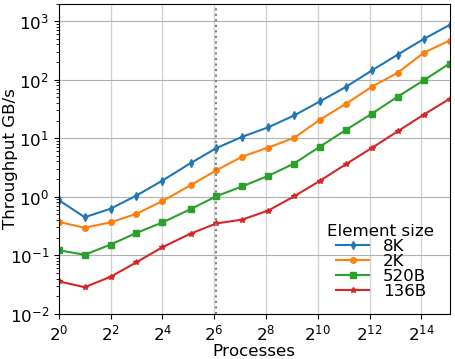
\includegraphics[scale=0.75]{projects/2.3.1-PMR/2.3.1.14-UPCxx-GASNet/all-cori-knl-out-inserts-wait.png}
  \caption{Weak scaling of distributed hash table insertion on the KNL partition of NERSC's Cori platform. The dotted line represents the processes in one node.}
  \label{fig:dht}
\end{figure}



\paragraph{Recent Progress}

\begin{enumerate}
\item \textbf{Memory Kinds.}
Unified abstractions for 
transferring data back and forth between device (e.g. GPU) and host memory, possibly remote.
By unifying the means of expressing data transfer among the collective memories of a heterogeneous system with different memory kinds,
the abstractions enable ECP applications to utilize accelerators, which are necessary to attain peak performance on ECP platforms.
The design and abstraction enables eventual hardware offload (such as to GPUDirect) of device data transfers, support for which will be provided in the near future by GASNet-EX.

\item \textbf{Portability and Sustainability.}
%Ensure that UPC++ remains viable as new compiler versions are released into the ECP software stack. 
UPC++ benefits to productivity rely heavily on template meta-programming, using features added in C++11.
However not all relevant C++ compilers comply sufficiently with the C++11 standard, 
necessitating deployment of various work-arounds within the UPC++ implementation.
The past year has seen the addition of UPC++ support for seven new CPU/compiler pairs.
A UPC++ Spack package has also been added to the E4S PMR SDK (Section~\ref{subsubsect:e4s}).

\end{enumerate}

\paragraph{Next Steps}

\begin{enumerate}
\item \textbf{Performance.}
With the help of our stakeholders, we are identifying portions of the UPC++
implementation where performance tuning is most needed and/or beneficial.
A recent example is deployment of an optimized implementation for
RMA puts using target-side completion notification.

\item \textbf{Productivity.}
With the core API specification and implementation of UPC++ nearly complete, we
are shifting focus toward some productivity-oriented features.  These include
UPC++ serialization of non-trivial user types and a distributed array facility
for UPC++.

\item \textbf{Outreach.}
We have begun activities designed to strengthen collaboration with our
stakeholders (both current ones, and potential future ones).  This includes
holding training events for users of UPC++ and circulating working group
drafts of productivity features (above) to solicit feedback.

\end{enumerate}
